\documentclass[11pt,a4paper]{article}

% ── Packages ──────────────────────────────────────────────────────────────────
\usepackage[T1]{fontenc}
\usepackage[utf8]{inputenc}
\usepackage{lmodern}
\usepackage[a4paper, margin=2.5cm]{geometry}
\usepackage{amsmath}
\usepackage{amssymb}
\usepackage{booktabs}
\usepackage{longtable}
\usepackage{array}
\usepackage{tabularx}
\usepackage{multirow}
\usepackage{xcolor}
\usepackage{listings}
\usepackage{hyperref}
\usepackage{microtype}
\usepackage{parskip}
\usepackage{enumitem}
\usepackage{fancyhdr}
\usepackage{titlesec}
\usepackage{tcolorbox}
\usepackage{mdframed}
\usepackage{tikz}
\usetikzlibrary{trees, positioning, shapes.geometric, arrows.meta}

% ── Colours ───────────────────────────────────────────────────────────────────
\definecolor{coinblue}{RGB}{0,70,140}
\definecolor{tiplightblue}{RGB}{230,242,255}
\definecolor{warnlight}{RGB}{255,248,225}
\definecolor{codegray}{RGB}{248,248,248}
\definecolor{codeborder}{RGB}{200,200,200}
\definecolor{darkgreen}{RGB}{0,100,0}
\definecolor{darkred}{RGB}{140,0,0}

% ── Hyperref setup ────────────────────────────────────────────────────────────
\hypersetup{
  colorlinks = true,
  linkcolor  = coinblue,
  urlcolor   = coinblue,
  citecolor  = coinblue,
  pdftitle   = {CLP LP Solver Parameter Tuning Guide},
  pdfauthor  = {Based on COIN-OR CLP source code analysis},
  pdfsubject = {Linear Programming, Parameter Tuning},
}

% ── Listings (shell commands / parameter examples) ────────────────────────────
\lstdefinestyle{clicmd}{
  backgroundcolor = \color{codegray},
  basicstyle      = \ttfamily\small,
  breaklines      = true,
  frame           = single,
  rulecolor       = \color{codeborder},
  xleftmargin     = 6pt,
  xrightmargin    = 6pt,
  aboveskip       = 6pt,
  belowskip       = 6pt,
}
\lstset{style=clicmd}

% ── Tip / Warning boxes ───────────────────────────────────────────────────────
\newmdenv[
  backgroundcolor = tiplightblue,
  linecolor       = coinblue,
  linewidth       = 1.2pt,
  leftmargin      = 0pt,
  rightmargin     = 0pt,
  innerleftmargin = 8pt,
  innerrightmargin= 8pt,
  innertopmargin  = 6pt,
  innerbottommargin=6pt,
  skipabove       = 8pt,
  skipbelow       = 8pt,
]{tipbox}

\newmdenv[
  backgroundcolor = warnlight,
  linecolor       = orange!70!black,
  linewidth       = 1.2pt,
  leftmargin      = 0pt,
  rightmargin     = 0pt,
  innerleftmargin = 8pt,
  innerrightmargin= 8pt,
  innertopmargin  = 6pt,
  innerbottommargin=6pt,
  skipabove       = 8pt,
  skipbelow       = 8pt,
]{warnbox}

% ── Section formatting ────────────────────────────────────────────────────────
\titleformat{\section}
  {\large\bfseries\color{coinblue}}
  {\thesection}{1em}{}[\vspace{-2pt}\rule{\linewidth}{0.5pt}]

\titleformat{\subsection}
  {\normalsize\bfseries\color{coinblue!80!black}}
  {\thesubsection}{1em}{}

\titleformat{\subsubsection}
  {\normalsize\bfseries}
  {\thesubsubsection}{1em}{}

% ── Header / footer ──────────────────────────────────────────────────────────
\pagestyle{fancy}
\fancyhf{}
\fancyhead[L]{\small\color{gray} CLP Parameter Tuning Guide}
\fancyhead[R]{\small\color{gray} COIN-OR CLP / CBC}
\fancyfoot[C]{\small\thepage}
\renewcommand{\headrulewidth}{0.3pt}

% ── Convenience macros ────────────────────────────────────────────────────────
\newcommand{\param}[1]{\texttt{\textbf{#1}}}
\newcommand{\val}[1]{\texttt{#1}}
\newcommand{\src}[1]{\textcolor{gray}{\small[\texttt{#1}]}}
\newcommand{\default}[1]{\textcolor{darkgreen}{\texttt{#1}}}
\newcommand{\important}{\textcolor{darkred}{\textbf{$\star$}}}

% ── Column types for tables ───────────────────────────────────────────────────
\newcolumntype{P}[1]{>{\raggedright\arraybackslash}p{#1}}
\newcolumntype{C}[1]{>{\centering\arraybackslash}p{#1}}

% ─────────────────────────────────────────────────────────────────────────────
\begin{document}

\begin{titlepage}
  \centering
  \vspace*{2cm}
  {\Huge\bfseries\color{coinblue} CLP Linear Programming Solver\\[0.4em]
   \Large Parameter Tuning Guide\par}
  \vspace{1.5em}
  {\large COIN-OR CLP / CBC\par}
  \vspace{0.5em}
  {\normalsize Based on source-code analysis of CLP\par}
  \vspace{0.3em}
  {\normalsize and the empirical study by Vilas Boas et al.\ (ITOR 2019)\par}
  \vspace{3cm}
  \begin{mdframed}[backgroundcolor=tiplightblue, linecolor=coinblue, linewidth=1pt]
    \centering\small
    Sources: \texttt{ClpParameters.cpp}, \texttt{ClpModel.cpp},
    \texttt{ClpSimplex\{Dual,Primal\}.cpp},\\
    \texttt{ClpInterior.cpp}, \texttt{ClpSolve.cpp},
    \texttt{CbcOrClpParam.cpp}, \texttt{Cbc\_C\_Interface.cpp},\\
    \texttt{ClpSimplexOther.cpp} (the \texttt{guess()} function), and
    \texttt{Osi/OsiFeatures.cpp}.
  \end{mdframed}
  \vfill
  {\small\color{gray}
    The $\important$ symbol marks high-impact parameters.\\
    Default values shown in \default{green monospace}.
  }
\end{titlepage}

\tableofcontents
\newpage

% =============================================================================
\section{Overview of CLP's LP Solvers}
\label{sec:overview}
% =============================================================================

CLP provides three LP algorithms, selectable via the \param{-duals}, \param{-primals},
and \param{-barrier} switches (or via \val{LPM\_Dual}/\val{LPM\_Primal}/\val{LPM\_Barrier}
in the C API).

\begin{center}
\begin{tabular}{@{}P{3cm}P{4cm}P{4.5cm}P{3cm}@{}}
  \toprule
  \textbf{Method} & \textbf{Default use} & \textbf{Strengths} & \textbf{Weaknesses} \\
  \midrule
  \textbf{Dual Simplex} & Root LP + every B\&B node & Warm-start from parent basis; fast for LP relaxations & Can be slow on degenerate problems \\
  \addlinespace
  \textbf{Primal Simplex} & Alternative; crash heuristics available & Better on structured / homogeneous problems; good with idiot crash & No warm-start from dual basis \\
  \addlinespace
  \textbf{Barrier (IPM)} & Large or difficult root LPs & Scales well; not affected by degeneracy & Requires crossover; no warm-start; expensive Cholesky \\
  \bottomrule
\end{tabular}
\end{center}

\subsection{How the default algorithm is selected}

When \param{-solve} is invoked via the C API with \val{LPM\_Auto}, CLP calls
\texttt{ClpSimplexOther::guess()} \src{ClpSimplexOther.cpp:11037}, a simple heuristic
that looks only at \textit{objective coefficient statistics}:

\begin{lstlisting}
sort objective coefficients; compute median(obj) and average(obj)
allInt = all bounded columns are flagged as integer?

if allInt:
    if average <= 0.0086207:  ->  Primal + idiot=30 + pertv=-1483
    else:                      ->  Primal + idiot=60
else:
    if median <= 0.75:         ->  Dual + PEsteepest + psi=1.0 + pertv=52
    else:                      ->  Primal + idiot=80
\end{lstlisting}

The empirical study (Section~\ref{sec:paper}) shows that the most important
discriminating feature is actually the \emph{constraint matrix coefficient range}
(\texttt{aRatioLSA}), which \texttt{guess()} does not consider.

% =============================================================================
\section{Parameters Common to All Solvers}
\label{sec:common}
% =============================================================================

\subsection{\important\ Scaling --- \param{-scaling}}

\begin{tabular}{@{}ll@{}}
  \textbf{Default:} & \default{automatic} \\
  \textbf{Options:} & \val{off}, \val{equilibrium}, \val{geometric}, \val{automatic},
                      \val{dynamic}, \val{rowsonly} \\
  \textbf{Source:}  & \src{ClpParameters.cpp, ClpModel.cpp}
\end{tabular}

\medskip
Scaling transforms the problem so that row and column magnitudes are more uniform,
reducing numerical errors and often the iteration count.

\begin{itemize}[noitemsep]
  \item \val{geometric} --- scales by $\sqrt{\max \times \min}$ per row/column.
        Often best for ill-conditioned matrices. Confirmed important by the paper.
  \item \val{equilibrium} --- scales by row/column maximum. Cheaper to compute.
  \item \val{automatic} --- CLP picks the method that minimises element ratio.
  \item \val{dynamic} --- rescales at every factorisation. Expensive but may help
        extreme cases.
  \item \val{off} --- best for numerically clean problems; eliminates unscaling
        overhead.
  \item \val{rows} (or \val{rowsonly}) --- scales rows only; tested in the paper
        for dual simplex on structured instances.
\end{itemize}

\begin{tipbox}
  \textbf{Recommendation:} leave \val{automatic} for general use.
  Try \val{-scaling geo} for ill-conditioned matrices (\texttt{aRatioLSA} $> 65$).
  The paper found \val{rows} scaling optimal for a cluster of degenerate dual problems.
\end{tipbox}

% ─────────────────────────────────────────────────────────────────────────────
\subsection{\important\ Presolve --- \param{-presolve} and \param{-passPresolve}}

\begin{tabular}{@{}ll@{}}
  \textbf{Default:} & \default{on} (5 passes) \\
  \textbf{Options:} & \val{on}, \val{more} (10 passes), \val{off} \\
  \textbf{passPresolve range:} & $[-200, 100]$, default \default{5} \\
  \textbf{Source:}  & \src{ClpParameters.cpp:1356}
\end{tabular}

\medskip
Presolve removes redundant constraints, fixes variables, and tightens bounds.
The \param{-passPresolve} integer parameter overrides the default number of passes;
negative values from the paper (e.g.\ $-81$) reduce the pass count below the default,
which can speed up B\&B nodes where presolve gains are modest.

\begin{tipbox}
  \textbf{Recommendation:} use \val{more} or \val{-passPresolve 20} for large,
  structured root LPs. Use \val{-passPresolve -33} or \val{off} for fast B\&B
  sub-problems. The paper found values of $\{-81, -67, -33, 0, 36, 67\}$ optimal
  for different instance classes.
\end{tipbox}

% ─────────────────────────────────────────────────────────────────────────────
\subsection{\important\ Substitution limit --- \param{-substitution}}

\begin{tabular}{@{}ll@{}}
  \textbf{Default:} & \default{3} \\
  \textbf{Range:}   & $[0,\,10000]$ \\
  \textbf{Source:}  & \src{ClpParameters.cpp:1400}
\end{tabular}

\medskip
Controls the maximum column length for presolve substitution. A value of $k$ means
presolve will substitute out any column with at most $k$ non-zeros. Higher values
produce more aggressive presolve (fewer rows/columns after presolve, but more
fill-in in the remaining matrix).

\begin{tipbox}
  \textbf{Recommendation:} the paper found \val{subs=4354} (extremely aggressive)
  optimal for a class of dual-simplex instances, at the cost of dense post-presolve
  matrix. Typical useful range: $\{3, 50, 138, 294\}$.
\end{tipbox}

% ─────────────────────────────────────────────────────────────────────────────
\subsection{\important\ Refactorisation frequency --- \param{-maxFactor}}

\begin{tabular}{@{}ll@{}}
  \textbf{Default:} & \default{200} (auto-tuned) \\
  \textbf{Auto-formula:} & $75 + \lfloor\text{rows}/50\rfloor$, capped at $1000$ \\
  \textbf{Source:}  & \src{ClpSimplex.cpp:11315 (defaultFactorizationFrequency())}
\end{tabular}

\medskip
The LU basis is refactorised every \param{maxFactor} pivots. Low values increase
numerical stability at the cost of more (expensive) factorisations. High values
reduce factorisation overhead but accumulate round-off.
CLP auto-tunes this by problem size when left at the default of $200$.

\begin{tipbox}
  \textbf{Recommendation:} leave at \val{200} (triggers auto-tune). For numerically
  difficult problems try $50$--$100$. For well-conditioned large problems try $400$--$1000$.
\end{tipbox}

% ─────────────────────────────────────────────────────────────────────────────
\subsection{Tolerances --- \param{-dualTolerance}, \param{-primalTolerance}}

\begin{tabular}{@{}ll@{}}
  \textbf{Defaults:} & \default{1e-7} (parameter file) / \default{1e-6} (runtime) \\
  \textbf{Source:}  & \src{ClpModel.cpp:132--133}
\end{tabular}

\medskip
\param{dualTolerance}: a variable is considered dual-feasible if its reduced cost
satisfies $|rc| \le \varepsilon_d$. \param{primalTolerance}: a constraint is
considered satisfied if its violation is below $\varepsilon_p$.

\begin{warnbox}
  Tightening tolerances below $10^{-8}$ can cause numerical cycling on
  ill-conditioned problems. If solutions appear slightly infeasible, \emph{loosen}
  to $10^{-6}$ rather than tighten.
\end{warnbox}

% ─────────────────────────────────────────────────────────────────────────────
\subsection{Sparse factorisation --- \param{-sparseFactor}}

\begin{tabular}{@{}ll@{}}
  \textbf{Default:} & \default{on} \\
  \textbf{Options:} & \val{on}, \val{off} \\
  \textbf{Source:}  & \src{ClpParameters.cpp:1520}
\end{tabular}

\medskip
When \val{off}, the LU factorisation is treated as dense. Normally this is slower,
but the paper found \val{spars=off} optimal for one cluster of instances where
aggressive presolve substitution (\val{subs=4354}) had already densified the matrix.

% ─────────────────────────────────────────────────────────────────────────────
\subsection{Dual reformulation --- \param{-dualize}}

\begin{tabular}{@{}ll@{}}
  \textbf{Default:} & \default{0} (off) \\
  \textbf{Options:} & \val{0}=off, \val{1}=always, \val{2}=if rows$>$cols, \val{4}=always \\
  \textbf{Source:}  & \src{ClpParameters.cpp:1322}
\end{tabular}

\medskip
Transposes the problem and solves the LP dual directly. Useful when the problem has
many more constraints than variables (tall matrix), so the dual has far fewer rows.
The paper evaluated \val{dualize=1} as one of the configurations for dual simplex instances.

% =============================================================================
\section{Dual Simplex Parameters}
\label{sec:dual}
% =============================================================================

The dual simplex is CBC's default LP solver. It solves the LP by maintaining dual
feasibility and driving primal infeasibilities to zero.

\subsection{\important\ Dual pivot rule --- \param{-dualPivot}}

\begin{tabular}{@{}ll@{}}
  \textbf{Default:} & \default{automatic} (= \texttt{ClpDualRowSteepest(mode=3)}) \\
  \textbf{Options:} & \val{automatic}, \val{dantzig}, \val{partial}, \val{steep},
                      \val{PEsteepest}, \val{PEdantzig} \\
  \textbf{Source:}  & \src{ClpDualRowSteepest.hpp, CbcSolver.cpp:2751}
\end{tabular}

\medskip
The pivot rule selects which leaving variable (row) enters the basis at each iteration.

\begin{center}
\begin{tabular}{@{}P{2.5cm}P{1.5cm}P{7.5cm}@{}}
  \toprule
  \textbf{Option} & \textbf{Mode} & \textbf{Description} \\
  \midrule
  \val{automatic} & 3 & Partial pricing, adaptive to full steepest edge
                        (default constructor \texttt{ClpDualRowSteepest(3)}) \\
  \val{dantzig}   & — & Largest reduced cost; simple but slow on large problems \\
  \val{partial}   & 2 & Partial steepest edge, uninitialized weights \\
  \val{steep}     & 1 & Full steepest edge (best anti-degeneracy, most computation) \\
  \val{PEsteepest}& 3+PE & Positive Edge steepest edge with compatible-variable
                            prioritisation (see Section~\ref{sec:psi}) \\
  \val{PEdantzig} & —+PE & Positive Edge Dantzig \\
  \bottomrule
\end{tabular}
\end{center}

\medskip
The \val{steep} (full steepest edge) maintains exact dual weights and is the strongest
anti-degeneracy rule. \val{PEsteepest} adds the Positive Edge criterion on top.

\begin{lstlisting}
# Use PEsteepest with moderate PE aggressiveness
clp problem.lp -dualPivot PEsteepest -psi 0.5 -duals
\end{lstlisting}

% ─────────────────────────────────────────────────────────────────────────────
\subsection{\important\ Positive Edge parameter --- \param{-psi}}
\label{sec:psi}

\begin{tabular}{@{}ll@{}}
  \textbf{CLI default:} & \default{$-0.5$} (PE inactive in auto mode) \\
  \textbf{Constructor default (\texttt{PEsteepest}):} & \default{$0.5$} \\
  \textbf{Range:}       & $(-1.1,\; 1.1)$ \\
  \textbf{Source:}      & \src{ClpPEDualRowSteepest.hpp, CbcOrClpParam.cpp:3591}
\end{tabular}

\medskip
The Positive Edge (PE) criterion \cite{Towhidi2014} prioritises \emph{compatible}
variables (those likely to make progress towards optimality) at each pivot.
The parameter $\psi$ controls the aggressiveness:

\begin{itemize}[noitemsep]
  \item $\psi \ge 1.0$ --- PE completely disabled; reverts to standard steepest edge.
        The compatible-variable check is skipped entirely
        \src{ClpPEDualRowSteepest.cpp:357}.
  \item $0 < \psi < 1.0$ --- PE active: a compatible row is preferred if
        $\text{largestComp} \ge \psi \cdot \text{largestIncompat}$.
        Smaller $\psi$ = more aggressive (always prefer compatible).
  \item $\psi < 0$ --- PE active; selection criterion becomes
        $\text{largestComp} \ge |\psi| \cdot \text{largestIncompat}$.
        The sign has no algorithmic effect once \val{PEsteepest} is selected.
\end{itemize}

\textbf{Two activation paths:}
\begin{enumerate}[noitemsep]
  \item \texttt{-dualPivot PEsteepest} alone $\Rightarrow$ PE active with
        $\psi = \texttt{fabs}(\text{CLI psi}) = 0.5$.
  \item \texttt{-psi 0.1} (positive, without explicit PEsteepest) $\Rightarrow$
        PE active for \emph{both} primal and dual with $\psi = 0.1$.
\end{enumerate}

\begin{tipbox}
  \textbf{Recommendation:} \val{-dualPivot PEsteepest -psi 0.1} for highly
  degenerate problems. The paper found \val{psi=1.0} (PE disabled) as the optimal
  configuration for some clusters --- suggesting that plain steepest edge can
  be better when the coefficient range is large.
\end{tipbox}

\begin{warnbox}
  \textbf{C-API bug in \texttt{Cbc\_C\_Interface.cpp:1897}:} the auto-tuner
  (\texttt{guess()}) writes the psi value to \texttt{int\_param[DBL\_PARAM\_PSI]}
  instead of \texttt{dbl\_param[DBL\_PARAM\_PSI]}. As a result the intended
  \texttt{psi=1.0} is never applied; the default \texttt{dbl\_param[DBL\_PARAM\_PSI] = -1.0}
  is used instead, producing maximally aggressive PE (any compatible row always wins).
\end{warnbox}

% ─────────────────────────────────────────────────────────────────────────────
\subsection{\important\ Dual bound --- \param{-dualBound}}

\begin{tabular}{@{}ll@{}}
  \textbf{Runtime default:} & \default{$10^{10}$} (set in \texttt{ClpModel} constructor) \\
  \textbf{Parameter default:} & \default{$0$} (maps to $10^{10}$ at solve time) \\
  \textbf{Range:}  & $[10^{-20},\; 10^{20}]$ \\
  \textbf{Source:} & \src{ClpModel.cpp:61}
\end{tabular}

\medskip
Bounds the magnitude of dual variables. Any dual variable exceeding this bound is
treated as if at its bound, effectively converting unbounded dual variables to
finite ones. This prevents the dual from becoming ill-conditioned but can cause
the LP to appear infeasible if set too tight.

\begin{tipbox}
  \textbf{Recommendation:} reduce to $10^{6}$--$10^{8}$ for ill-conditioned problems
  to improve numerical stability. Values around $10^{9}$ balance stability and
  accuracy. Leave at $10^{10}$ for well-conditioned problems.
\end{tipbox}

% ─────────────────────────────────────────────────────────────────────────────
\subsection{\important\ Perturbation --- \param{-perturbation} and \param{-pertValue}}

\begin{tabular}{@{}ll@{}}
  \textbf{Default (\texttt{perturbation\_}):} & \default{100} (auto perturbation on) \\
  \textbf{pertValue range:} & $[-5000,\; 102]$, default \default{50} \\
  \textbf{Source:}  & \src{ClpModel.cpp:113, ClpSimplexDual.cpp:6379}
\end{tabular}

\medskip
Perturbation adds small random noise to cost coefficients to break degeneracy.
The two parameters interact:

\paragraph{\param{-perturbation} (coarse control)}
\begin{itemize}[noitemsep]
  \item \val{50} --- no perturbation (but CLP may still perturb automatically
        if it detects degenerate objectives).
  \item \val{100} --- automatic perturbation (default). CLP decides when to perturb.
  \item \val{101} / \val{102} --- already perturbed / stop further perturbation.
\end{itemize}

\paragraph{\param{-pertValue} (fine-grained control, $[-5000, 102]$)}
Values $51$--$61$ select the maximum perturbation fraction from a lookup table
($m[\text{pertValue} - 51]$):

\begin{center}
\begin{tabular}{@{}ccl@{}}
  \toprule
  \textbf{pertValue} & \textbf{maxFraction} & \textbf{Effect} \\
  \midrule
  50  & auto    & Standard auto-perturbation \\
  51  & $10^{-10}$ & Minimal perturbation \\
  52  & $10^{-9}$  & Very conservative (used with PEsteepest by \texttt{guess()}) \\
  56  & $10^{-5}$  & Moderate \\
  61  & $1.0$      & Large perturbation \\
  \bottomrule
\end{tabular}
\end{center}

Negative values activate a more complex encoding: values $\le -900$ also perturb
row costs; values with tens-digit $\ge 1$ activate uniform perturbation.
For example, \val{pertValue=-1483} (used by \texttt{guess()} for all-integer primal)
encodes: row-cost perturbation + uniform change + $\text{maxFraction} = 10^{-5}$.

\begin{tipbox}
  \textbf{Recommendation:} use \val{-pertValue 52} with \val{PEsteepest}
  (conservative, lets PE handle degeneracy). Try \val{-pertValue 56} or \val{61}
  for strongly degenerate primal problems. For the paper's leaf L5 configuration,
  \val{pertValue=81} was optimal.
\end{tipbox}

% ─────────────────────────────────────────────────────────────────────────────
\subsection{Dual crash --- \param{-crash}}

\begin{tabular}{@{}ll@{}}
  \textbf{Default:} & \default{off} \\
  \textbf{Options:} & \val{off}, \val{on}, \val{solow}, \val{lots}, \val{idiot1}--\val{idiot7} \\
  \textbf{Source:}  & \src{ClpParameters.cpp}
\end{tabular}

\medskip
An initial basis construction heuristic. For dual simplex, the paper found
\val{crash=idiot6} (6 passes of the idiot heuristic as warm-start) optimal
for a specific class of degenerate instances. This is unusual since idiot is
normally a primal preprocessing technique.

% =============================================================================
\section{Primal Simplex Parameters}
\label{sec:primal}
% =============================================================================

The primal simplex maintains primal feasibility and drives dual infeasibilities
to zero. Best when a good primal-feasible starting point is available or after
idiot crash.

\subsection{\important\ Idiot crash --- \param{-idiot}}

\begin{tabular}{@{}ll@{}}
  \textbf{Default:} & \default{$-1$} (auto; use only if problem is suitable) \\
  \textbf{Range:}   & $[-1,\; \infty)$; $0$ = off, $n > 0$ = $n$ passes \\
  \textbf{Source:}  & \src{ClpParameters.cpp:1322}
\end{tabular}

\medskip
The idiot heuristic runs a conjugate-gradient-like method (similar to MINOS's
crash) that produces a near-primal-feasible starting point before the simplex.
It is most effective on \emph{homogeneous} problems with unit elements and
structured RHS (e.g.\ network-flow, binary LPs).

\begin{center}
\begin{tabular}{@{}cl@{}}
  \toprule
  \textbf{Value} & \textbf{When optimal (from paper)} \\
  \midrule
  7   & Well-conditioned, near-uniform objective, no integer structure \\
  30  & All-integer problems, very small average objective \\
  60  & All-integer problems, moderate objective \\
  80  & Continuous LPs with median objective $> 0.75$ \\
  100 & Ill-conditioned problems with large objective range \\
  \bottomrule
\end{tabular}
\end{center}

\begin{tipbox}
  \textbf{Recommendation:} \val{-idiot 60} is a strong default for primal simplex
  on structured MIP LPs. Try values from $\{7, 30, 60, 80, 100\}$.
\end{tipbox}

% ─────────────────────────────────────────────────────────────────────────────
\subsection{\important\ Sprint crash --- \param{-sprint}}

\begin{tabular}{@{}ll@{}}
  \textbf{Default:} & \default{$-1$} (auto; off on most problems) \\
  \textbf{Range:}   & $[-1,\; \infty)$; $0$ = off, $n > 0$ = $n$ columns per sprint \\
  \textbf{Source:}  & \src{ClpParameters.cpp:1390}
\end{tabular}

\medskip
Sprint (also called \emph{sifting} in CPLEX) is designed for \emph{long and thin}
problems --- many more columns than rows. CLP solves a sequence of restricted LPs
each using a subset of $n$ columns, cycling through the full column set.

\begin{tipbox}
  \textbf{Recommendation:} try \val{-sprint 1217} or \val{-sprint 3384} on
  problems with $\text{cols} \gg \text{rows}$ (e.g.\ cutting stock, multi-commodity
  flow). Values $\{1217, 1557, 1804, 3384, 4826\}$ were explored in the paper.
\end{tipbox}

% ─────────────────────────────────────────────────────────────────────────────
\subsection{Primal pivot rule --- \param{-primalPivot}}

\begin{tabular}{@{}ll@{}}
  \textbf{Default:} & \default{automatic} (= \texttt{ClpPrimalColumnSteepest(mode=3)}) \\
  \textbf{Options:} & \val{automatic}, \val{exact}, \val{dantzig}, \val{partial},
                      \val{change}, \val{sprint}, \val{PEsteepest} \\
  \textbf{Source:}  & \src{ClpPrimalColumnSteepest.hpp, CbcSolver.cpp:2784}
\end{tabular}

\medskip
\begin{center}
\begin{tabular}{@{}P{2.5cm}P{1.5cm}P{7.5cm}@{}}
  \toprule
  \textbf{Option} & \textbf{Mode} & \textbf{Description} \\
  \midrule
  \val{automatic} & 3 & Adaptive devex (partial $\to$ full) \\
  \val{exact}     & 0 & Exact devex weights \\
  \val{dantzig}   & — & Largest reduced cost \\
  \val{partial}   & 4 & Partial pricing, dantzig/devex $\to$ adaptive \\
  \val{change}    & 1 & Full steepest edge \\
  \val{sprint}    & 10 & Sprint-based column selection \\
  \val{PEsteepest}& +PE & Positive Edge steepest edge \\
  \bottomrule
\end{tabular}
\end{center}

% ─────────────────────────────────────────────────────────────────────────────
\subsection{Primal weight --- \param{-primalWeight} / \texttt{infeasibilityCost}}

\begin{tabular}{@{}ll@{}}
  \textbf{Default:} & \default{$10^{10}$} (internal; parameter default $10^{10}$) \\
  \textbf{Source:}  & \src{ClpParameters.cpp, ClpSimplexPrimal.cpp}
\end{tabular}

\medskip
The primal simplex uses a big-$M$ penalty (\texttt{infeasibilityCost}) to handle
infeasibility. This value controls the relative importance of reducing infeasibility
vs.\ improving the objective. Increasing it makes CLP more aggressive in reaching
primal feasibility.

% =============================================================================
\section{Barrier (Interior Point) Method Parameters}
\label{sec:barrier}
% =============================================================================

The barrier method uses a primal-dual interior point algorithm. It does not
maintain a basis and typically requires a crossover step to recover an optimal
simplex basis.

\subsection{\important\ Cholesky factorisation --- \param{-cholesky}}

\begin{tabular}{@{}ll@{}}
  \textbf{Default:} & \default{native} \\
  \textbf{Options:} & \val{native}, \val{dense}, \val{UniversityOfFlorida},
                      \val{Mumps}, \val{Wssmp} \\
  \textbf{Source:}  & \src{ClpSolve.cpp:3140--3330 (cholesky case switch)}
\end{tabular}

\medskip
The Cholesky factorisation is the dominant cost at each barrier iteration.
\val{UniversityOfFlorida} uses the AMD (Approximate Minimum Degree) ordering
from the SuiteSparse library, which dramatically reduces fill-in for
sparse problems.

\begin{tipbox}
  \textbf{If compiled with AMD/SuiteSparse:} always use
  \val{-cholesky UniversityOfFlorida}. It was the only non-native option
  in the paper's barrier experiments, confirming its importance.
  Note: with CHOLMOD available, CLP forces \texttt{supernodal=0}
  because barrier matrices may not be positive definite in early iterations.
\end{tipbox}

% ─────────────────────────────────────────────────────────────────────────────
\subsection{Regularisation --- \param{-gamma} and \param{-delta}}

\begin{tabular}{@{}ll@{}}
  \textbf{Defaults:} & \default{$\gamma = 0$}, \default{$\delta = 0$} \\
  \textbf{Source:}   & \src{ClpInterior.cpp:61--62, ClpSolve.cpp:3290}
\end{tabular}

\medskip
$\gamma$ and $\delta$ are regularisation parameters for the barrier normal equations.
They prevent the KKT matrix from becoming singular near the boundary of the feasible
region (ill-conditioned / near-degenerate problems).
They are set via \param{-gamma} and implicitly via the \param{aggressiveGamma} bitfield
in \texttt{ClpSolve}:

\begin{center}
\begin{tabular}{@{}clll@{}}
  \toprule
  \textbf{Level} & \textbf{$\gamma$} & \textbf{$\delta$} & \textbf{When to use} \\
  \midrule
  off (default) & $0$         & $0$         & Well-conditioned problems \\
  1             & $10^{-5}$   & $10^{-5}$   & Mild ill-conditioning \\
  2             & $10^{-7}$   & $0$         & Near-degenerate primal \\
  3             & $0$         & $10^{-5}$   & Near-degenerate dual \\
  4             & $10^{-3}$   & $10^{-3}$   & Strong regularisation \\
  \bottomrule
\end{tabular}
\end{center}

% ─────────────────────────────────────────────────────────────────────────────
\subsection{Crossover --- \param{-crossover}}

\begin{tabular}{@{}ll@{}}
  \textbf{Default:} & \default{on} \\
  \textbf{Options:} & \val{on}, \val{off}, \val{maybe} \\
  \textbf{Source:}  & \src{ClpSolve.cpp}
\end{tabular}

\medskip
After barrier convergence, crossover moves from the interior point solution to
a vertex of the optimal face (a basic feasible solution). This is required for:
\begin{itemize}[noitemsep]
  \item Warm-starting subsequent dual simplex iterations (e.g.\ B\&B nodes).
  \item Sensitivity analysis (requires a basis).
\end{itemize}

Use \val{off} if only the optimal objective value and primal solution are needed
(not a basis), saving potentially significant computation.

% ─────────────────────────────────────────────────────────────────────────────
\subsection{Barrier iteration limit --- \param{-maxIterations}}

\begin{tabular}{@{}ll@{}}
  \textbf{Default:} & \default{200} (raised to \default{1000} if rows+cols $>$ 10000) \\
  \textbf{Source:}  & \src{ClpInterior.cpp:103}
\end{tabular}

% ─────────────────────────────────────────────────────────────────────────────
\subsection{Barrier perturbation --- \param{-pertValue} (barrier context)}

The paper tested barrier-specific \param{pertValue} values:
$\{-208, -61, 50, 51, 56, 61, 102, 208\}$.
The same encoding as the dual simplex applies. Values $51$--$56$ are conservative;
$102$ stops further perturbation; negative values encode complex perturbation
patterns including row-cost modification.

% =============================================================================
\section{Summary Tables}
\label{sec:tables}
% =============================================================================

\subsection{All parameters at a glance}

\begin{longtable}{@{}P{3.5cm}P{2.5cm}P{2.2cm}P{5cm}@{}}
  \toprule
  \textbf{Parameter} & \textbf{Default} & \textbf{Solver} & \textbf{Tuning suggestion} \\
  \midrule
  \endhead
  \midrule
  \multicolumn{4}{r}{\small (continues\ldots)} \\
  \endfoot
  \bottomrule
  \endlastfoot

  % Common
  \param{scaling}       & \val{automatic}  & All & \val{geo} (ill-cond.), \val{rows} (structured dual) \\
  \param{presolve}      & \val{on}          & All & \val{more} for root LP \\
  \param{passPresolve}  & \val{5}           & All & $\{-81,-33,20,80\}$ \\
  \param{substitution}  & \val{3}           & All & $\{50, 138, 4354\}$ \\
  \param{maxFactor}     & \val{200} (auto)  & All & $\{50\text{--}200, 400\text{--}1000\}$ \\
  \param{dualTolerance} & \val{1e-6}        & All & loosen to \val{1e-5} if unstable \\
  \param{primalTolerance}& \val{1e-6}       & All & loosen to \val{1e-5} if unstable \\
  \param{sparseFactor}  & \val{on}          & All & \val{off} after aggressive \val{subs} \\
  \param{dualize}       & \val{0}           & Dual/Primal & \val{2} (rows$\gg$cols) \\
  \addlinespace
  % Dual
  \param{dualPivot}     & \val{automatic}   & Dual & \val{PEsteepest} (\important) \\
  \param{psi}           & \val{-0.5}        & Dual/Primal & $\{0.1, 0.5\}$ (PE active); \val{1.0} (PE off) \\
  \param{dualBound}     & \val{1e10}        & Dual & $\{10^6,10^8,10^9\}$ (ill-cond.) \\
  \param{perturbation}  & \val{100}         & Dual & \val{50} (off), \val{100} (auto) \\
  \param{pertValue}     & \val{50}          & Dual & \val{52} (w/ PEsteepest), \val{56}, \val{81} \\
  \param{crash}         & \val{off}         & Dual & \val{idiot6} (degenerate) \\
  \addlinespace
  % Primal
  \param{idiot}         & \val{-1}          & Primal & $\{7, 30, 60, 80, 100\}$ (\important) \\
  \param{sprint}        & \val{-1}          & Primal & $\{1217, 3384\}$ (cols$\gg$rows) \\
  \param{primalPivot}   & \val{automatic}   & Primal & \val{PEsteepest} (degenerate) \\
  \param{primalWeight}  & \val{1e10}        & Primal & increase if many infeasibilities \\
  \addlinespace
  % Barrier
  \param{cholesky}      & \val{native}      & Barrier & \val{UniversityOfFlorida} (\important) \\
  \param{gamma}         & \val{0}           & Barrier & levels $1$--$4$ (ill-cond.) \\
  \param{crossover}     & \val{on}          & Barrier & \val{off} (no basis needed) \\
  \param{maxIterations} & \val{200/1000}    & Barrier & $\{500, 2000\}$ \\
  \param{pertValue}     & \val{50}          & Barrier & $\{51,56,61,102,-208\}$ \\
\end{longtable}

% =============================================================================
\section{Empirical Study: Decision Trees for Algorithm Selection}
\label{sec:paper}
% =============================================================================

Vilas Boas, Santos et al.~\cite{VBoas2019} evaluated 532 CLP configurations on
1004 LP instances (all MIPLIB benchmarks, LP relaxations) and used integer
programming to construct optimal decision trees for algorithm selection.
Key results: 22\% improvement with the single best configuration over CLP defaults;
40\% improvement using the full depth-3 decision tree (cross-validated).

\subsection{Most discriminating problem features}

The features that appear at the root and high levels of the optimal decision tree
are the \emph{strongest predictors} of the best algorithm.

\begin{center}
\begin{tabular}{@{}P{3cm}P{5.5cm}P{5cm}@{}}
  \toprule
  \textbf{Feature} & \textbf{Description} & \textbf{Why it matters} \\
  \midrule
  \texttt{aRatioLSA} \important & Ratio of largest to smallest absolute
    non-zero in constraint matrix &
    \textbf{Root split (most important).} High ratio = ill-conditioned matrix;
    favours primal. \\
  \addlinespace
  \texttt{objMed} & Median of objective coefficients &
    Near-zero median $\Rightarrow$ structured/near-degenerate objective;
    same as used by \texttt{guess()}. \\
  \addlinespace
  \texttt{rhsMax} & Maximum RHS value &
    Large RHS $\Rightarrow$ large dual feasible region; favours primal crash. \\
  \addlinespace
  \texttt{objRatioLSA} & Ratio of largest/smallest absolute objective coeff. &
    Measures objective conditioning; appears at level~3 (multiple nodes). \\
  \addlinespace
  \texttt{int} & Number of integer variables &
    LP relaxation context: separates pure-continuous from mixed instances. \\
  \bottomrule
\end{tabular}
\end{center}

\begin{warnbox}
  The \texttt{guess()} heuristic uses only \texttt{objMed}/\texttt{objAvg}, ignoring
  the most discriminating feature \texttt{aRatioLSA} (constraint matrix conditioning).
  For instance-specific tuning, compute \texttt{aRatioLSA}
  $= \max_{a_{ij}\neq 0}|a_{ij}| \,/\, \min_{a_{ij}\neq 0}|a_{ij}|$
  and use it to guide algorithm selection.
\end{warnbox}

\subsection{The depth-3 decision tree}

Figure~\ref{fig:tree} shows the structure of the paper's depth-3 decision tree with
8 leaf nodes covering all 1004 instances. Each leaf shows the recommended
algorithm configuration and number of instances assigned.

\begin{figure}[ht]
  \centering
  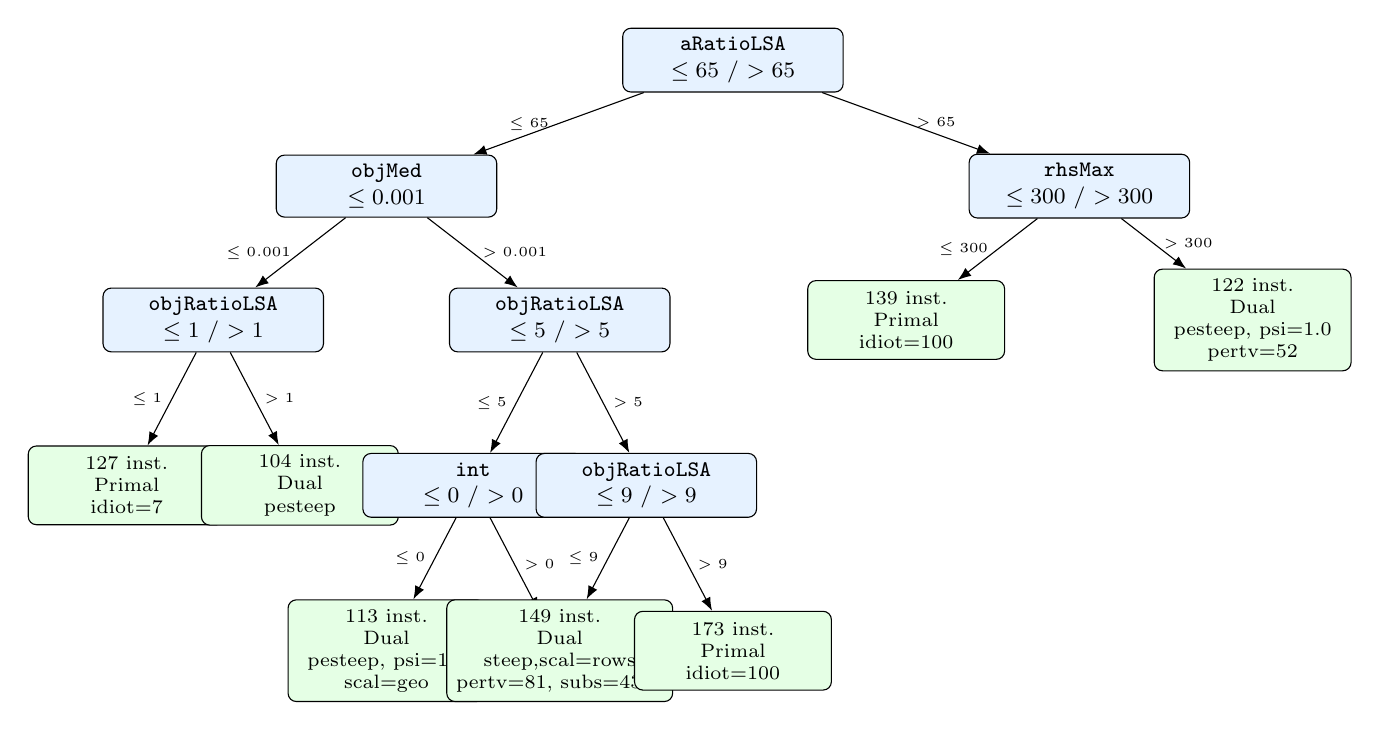
\begin{tikzpicture}[
      font=\footnotesize,
      every node/.style={align=center},
      inner/.style={draw, rounded corners=3pt, fill=tiplightblue,
                    minimum width=2.8cm, minimum height=0.7cm},
      leaf/.style={draw, fill=green!10, rounded corners=3pt,
                   minimum width=2.5cm, minimum height=1.0cm, font=\scriptsize},
      edge from parent/.style={draw, -Latex},
      level 1/.style={sibling distance=88mm, level distance=16mm},
      level 2/.style={sibling distance=44mm, level distance=17mm},
      level 3/.style={sibling distance=22mm, level distance=21mm},
    ]
    \node[inner] {\texttt{aRatioLSA}\\$\le 65$ / $> 65$}
      child {
        node[inner] {\texttt{objMed}\\$\le 0.001$}
        child {
          node[inner] {\texttt{objRatioLSA}\\$\le 1$ / $> 1$}
          child {
            node[leaf] {127 inst.\\Primal\\idiot=7}
            edge from parent node[left, font=\tiny] {$\le 1$}
          }
          child {
            node[leaf] {104 inst.\\Dual\\pesteep}
            edge from parent node[right, font=\tiny] {$> 1$}
          }
          edge from parent node[left, font=\tiny] {$\le 0.001$}
        }
        child {
          node[inner] {\texttt{objRatioLSA}\\$\le 5$ / $> 5$}
          child {
            node[inner] {\texttt{int}\\$\le 0$ / $> 0$}
            child {
              node[leaf] {113 inst.\\Dual\\pesteep, psi=1.0\\scal=geo}
              edge from parent node[left, font=\tiny] {$\le 0$}
            }
            child {
              node[leaf] {77 inst.\\Primal\\idiot=80}
              edge from parent node[right, font=\tiny] {$> 0$}
            }
            edge from parent node[left, font=\tiny] {$\le 5$}
          }
          child {
            node[inner] {\texttt{objRatioLSA}\\$\le 9$ / $> 9$}
            child {
              node[leaf] {149 inst.\\Dual\\steep,scal=rows\\pertv=81, subs=4354}
              edge from parent node[left, font=\tiny] {$\le 9$}
            }
            child {
              node[leaf] {173 inst.\\Primal\\idiot=100}
              edge from parent node[right, font=\tiny] {$> 9$}
            }
            edge from parent node[right, font=\tiny] {$> 5$}
          }
          edge from parent node[right, font=\tiny] {$> 0.001$}
        }
        edge from parent node[left, font=\tiny] {$\le 65$}
      }
      child {
        node[inner] {\texttt{rhsMax}\\$\le 300$ / $> 300$}
        child {
          node[leaf] {139 inst.\\Primal\\idiot=100}
          edge from parent node[left, font=\tiny] {$\le 300$}
        }
        child {
          node[leaf] {122 inst.\\Dual\\pesteep, psi=1.0\\pertv=52}
          edge from parent node[right, font=\tiny] {$> 300$}
        }
        edge from parent node[right, font=\tiny] {$> 65$}
      };
  \end{tikzpicture}
  \caption{Depth-3 decision tree for CLP algorithm selection (Vilas Boas et al.,
           ITOR 2019). 1004 LP relaxation instances; 40\% improvement over defaults
           in cross-validation. Internal nodes show the splitting feature and
           threshold; leaves show recommended algorithm configuration and instance count.}
  \label{fig:tree}
\end{figure}

\subsection{Configurations per leaf and parameters evaluated in Table~2}

\begin{center}
\begin{tabular}{@{}clP{9cm}@{}}
  \toprule
  \textbf{Instances} & \textbf{Method} & \textbf{Configuration} \\
  \midrule
  127 & Primal & \texttt{idiot=7} \\
  104 & Dual   & \texttt{dualp=pesteep} \\
  113 & Dual   & \texttt{dualp=pesteep, psi=1.0, scal=geo} \\
  77  & Primal & \texttt{idiot=80} \\
  149 & Dual   & \texttt{crash=idiot6, dualp=steep, scal=rows, spars=off,}
                 \texttt{subs=4354, pertv=81, passp=-81} \\
  173 & Primal & \texttt{idiot=100} \\
  139 & Primal & \texttt{idiot=100} \\
  122 & Dual   & \texttt{dualp=pesteep, psi=1.0, pertv=52} \\
  \bottomrule
\end{tabular}
\end{center}

\medskip
The paper explored the following ranges for each parameter (Table~2 of the paper):

\begin{center}
\begin{tabular}{@{}P{2.5cm}P{10.5cm}@{}}
  \toprule
  \textbf{Parameter} & \textbf{Values tested} \\
  \midrule
  \multicolumn{2}{@{}l}{\textit{Primal simplex}} \\
  \texttt{idiot}    & \{3,4,5,6,7,9,10,11\} \\
  \texttt{pertv}    & \{3500, $-3157$, $-3000$, $-2395$, $-2000$, $-1483$, $-1000$, 61\} \\
  \texttt{sprint}   & \{1217, 1557, 1804, 3384, 4826\} \\
  \texttt{primalp}  & \{change, exa(ct)\} \\
  \texttt{psi}      & \{$-0.84$, $-0.62$, $-0.35$, 0.62, 0.66, 0.84, 0.91\} \\
  \texttt{scal}     & \{geo, rows\} \\
  \texttt{subs}     & \{138, 294\} \\
  \texttt{perturb}  & \{1, 57, 15, 20, 25, 30, 35, 40, 50, 60, 80, 100\} \\
  \texttt{passp}    & \{22, 40, 80, 138, 294\} \\
  \addlinespace
  \multicolumn{2}{@{}l}{\textit{Dual simplex}} \\
  \texttt{idiot/crash} & \{idiot1\ldots 7, on, lots, so\} \\
  \texttt{dualize}  & \{1\} \\
  \texttt{pertv}    & \{4900, \ldots, 820\} (various including negatives) \\
  \texttt{dualp}    & \{pesteep, steep\} \\
  \texttt{psi}      & \{$-1.1$, \ldots, 1.1\} \\
  \texttt{scal}     & \{geo, rows\} \\
  \texttt{passp}    & \{167, $-81$, $-67$, $-33$, 0, 36, 67, 93\} \\
  \texttt{subs}     & \{37, 40, 41, 4354, 4392\} \\
  \addlinespace
  \multicolumn{2}{@{}l}{\textit{Barrier}} \\
  \texttt{cholesky} & \{UniversityOfFlorida, dense\} \\
  \texttt{pertv}    & \{$-208$, $-61$, 50, 51, 56, 61, 102, 208\} \\
  \bottomrule
\end{tabular}
\end{center}

% =============================================================================
\section{Practical Tuning Recommendations}
\label{sec:recs}
% =============================================================================

\subsection{Quick decision guide}

\begin{enumerate}
  \item \textbf{Compute \texttt{aRatioLSA}} = max absolute coefficient / min absolute
        coefficient in the constraint matrix.
  \begin{itemize}[noitemsep]
    \item $\text{aRatioLSA} \le 65$: matrix is well-conditioned $\to$ follow the
          left branch of Figure~\ref{fig:tree} (check \texttt{objMed}).
    \item $\text{aRatioLSA} > 65$: matrix is ill-conditioned $\to$ right branch
          (check \texttt{rhsMax}).
  \end{itemize}

  \item \textbf{For dual simplex on degenerate problems:}
\begin{lstlisting}
clp problem.lp -dualPivot PEsteepest -psi 0.1 -pertValue 52 \
               -scaling geo -duals
\end{lstlisting}

  \item \textbf{For primal simplex on structured/integer-heavy LPs:}
\begin{lstlisting}
clp problem.lp -idiot 60 -scaling geo -primals
\end{lstlisting}

  \item \textbf{For barrier (large or difficult root LP), with AMD build:}
\begin{lstlisting}
clp problem.lp -barrier -cholesky UniversityOfFlorida \
               -crossover on -scaling geo
\end{lstlisting}

  \item \textbf{For long/thin problems (many columns, few rows):}
\begin{lstlisting}
clp problem.lp -sprint 3384 -primals
\end{lstlisting}
\end{enumerate}

\subsection{Recommended parameter grid for instance-based tuning}

The following grids can be used as a starting point for automated tuning
(e.g.\ with irace or manual grid search):

\paragraph{Dual simplex}
\begin{lstlisting}
dualPivot  : {automatic, PEsteepest, steep}
psi        : {0.1, 0.5, 1.0}          # 1.0 = PE off
pertValue  : {50, 52, 56, 81}
scaling    : {automatic, geo, rows}
passPresolve: {5, -33, -67, -81}
substitution: {3, 138, 4354}
crash      : {off, idiot6}
\end{lstlisting}

\paragraph{Primal simplex}
\begin{lstlisting}
idiot      : {0, 7, 30, 60, 80, 100}
pertValue  : {50, 61, -1483}
sprint     : {0, 1217, 3384}
scaling    : {automatic, geo, rows}
passPresolve: {5, 40, 80, 138}
\end{lstlisting}

\paragraph{Barrier}
\begin{lstlisting}
cholesky   : {native, UniversityOfFlorida}
pertValue  : {50, 51, 56, 61, 102, -208}
gamma      : {off, on (level 1), onstrong (level 4)}
crossover  : {on, off}
\end{lstlisting}

\subsection{Notes for CBC branch-and-bound context}

\begin{enumerate}
  \item \textbf{Dual simplex at every B\&B node}: warm-start from parent basis.
        Parameters affecting dual convergence and stability are most critical.
        \val{PEsteepest} + modest \val{pertValue} is the highest-leverage setting.
  \item \textbf{\texttt{dualBound}} matters most at the root LP. Child-node LPs
        typically have tight bounds from branching, reducing the risk of large duals.
  \item \textbf{Barrier for root LP only}: no warm-start between nodes. Use
        \val{-cholesky UniversityOfFlorida -crossover on} for large root LPs.
  \item \textbf{Presolve effort at nodes}: reduce with \val{-passPresolve -33} or
        lower to avoid overhead at B\&B nodes where gains are small.
  \item \textbf{Idiot crash}: most beneficial for the first LP (root). Not useful
        at child nodes where a warm basis is available.
\end{enumerate}

% =============================================================================
\section{Default Values Reference}
\label{sec:defaults}
% =============================================================================

\begin{center}
\begin{tabular}{@{}P{4cm}P{3cm}P{7cm}@{}}
  \toprule
  \textbf{Parameter} & \textbf{Runtime default} & \textbf{Source location} \\
  \midrule
  \texttt{dualTolerance}         & $10^{-6}$            & \texttt{ClpModel.cpp:132} \\
  \texttt{primalTolerance}       & $10^{-6}$            & \texttt{ClpModel.cpp:133} \\
  \texttt{dualBound}             & $10^{10}$            & \texttt{ClpModel.cpp:61} \\
  \texttt{perturbation\_}        & $100$ (auto on)      & \texttt{ClpModel.cpp:113} \\
  \texttt{maxFactor}             & 200 $\to$ auto-tuned & \texttt{CoinFactorization1.cpp:217} \\
  auto-tune formula              & $75 + \lfloor n/50 \rfloor$, cap 1000 &
                                   \texttt{ClpSimplex.cpp:11315} \\
  \texttt{dualRowPivot}          & \texttt{ClpDualRowSteepest(mode=3)} &
                                   \texttt{ClpModel.cpp:157} \\
  \texttt{primalColPivot}        & \texttt{ClpPrimalColumnSteepest(mode=3)} & \\
  \texttt{scaling}               & automatic             & \texttt{ClpParameters.cpp} \\
  \texttt{presolve}              & on (5 passes)         & \texttt{ClpParameters.cpp} \\
  \texttt{substitution}          & 3                     & \texttt{ClpParameters.cpp:1400} \\
  \texttt{idiot}                 & $-1$ (auto)           & \texttt{ClpParameters.cpp} \\
  \texttt{sprint}                & $-1$ (auto)           & \texttt{ClpParameters.cpp} \\
  \texttt{psi} (CLI)             & $-0.5$ (PE inactive)  & \texttt{CbcOrClpParam.cpp:3592} \\
  \texttt{psi} (PEsteepest ctor) & $0.5$                 & \texttt{ClpPEDualRowSteepest.hpp} \\
  \texttt{psi} (C API default)   & $-1.0$                & \texttt{Cbc\_C\_Interface.cpp:4956} \\
  \midrule
  \multicolumn{3}{@{}l}{\textit{Barrier}} \\
  \texttt{gamma\_}               & $0.0$                 & \texttt{ClpInterior.cpp:61} \\
  \texttt{delta\_}               & $0.0$                 & \texttt{ClpInterior.cpp:62} \\
  \texttt{maxBarrierIterations}  & 200 ($\to$1000 if large) & \texttt{ClpInterior.cpp:103} \\
  \texttt{diagonalPerturbation}  & $10^{-15}$            & \texttt{ClpInterior.cpp:60} \\
  \texttt{projectionTolerance}   & $10^{-7}$             & \texttt{ClpInterior.cpp} \\
  \texttt{cholesky}              & native                & \texttt{ClpSolve.cpp:3140} \\
  \bottomrule
\end{tabular}
\end{center}

% =============================================================================
% Bibliography
% =============================================================================
\begin{thebibliography}{9}

\bibitem{VBoas2019}
  M.~G. Vilas Boas, H.~G. Santos, L.~H.~C. Merschmann, G.~Vanden Berghe,
  \textit{Optimal Decision Trees for the Algorithm Selection Problem:
  Integer Programming Based Approaches},
  International Transactions in Operational Research,
  DOI: 10.1111/itor.12724, 2019.

\bibitem{Towhidi2014}
  M.~Towhidi, J.~Orban, F.~Soumis,
  \textit{The positive edge simplex method for linear programming},
  INFORMS Journal on Computing 26(3):467--481, 2014.

\bibitem{CLP}
  COIN-OR Foundation,
  \textit{COIN-OR Linear Programming (CLP)},
  \url{https://github.com/coin-or/Clp}.

\bibitem{CBC}
  COIN-OR Foundation,
  \textit{COIN-OR Branch and Cut (CBC)},
  \url{https://github.com/coin-or/Cbc}.

\end{thebibliography}

\end{document}
